\documentclass[tikz]{standalone}
\usepackage{pgfplots}
\usepgfplotslibrary{groupplots}
\pgfplotsset{width=8cm, height=7cm, compat=1.18}
\usepackage{tikz}
\usepackage{amsmath}
\usetikzlibrary {arrows.meta} 
\newcommand{\mytau}{0.075}

\begin{document}

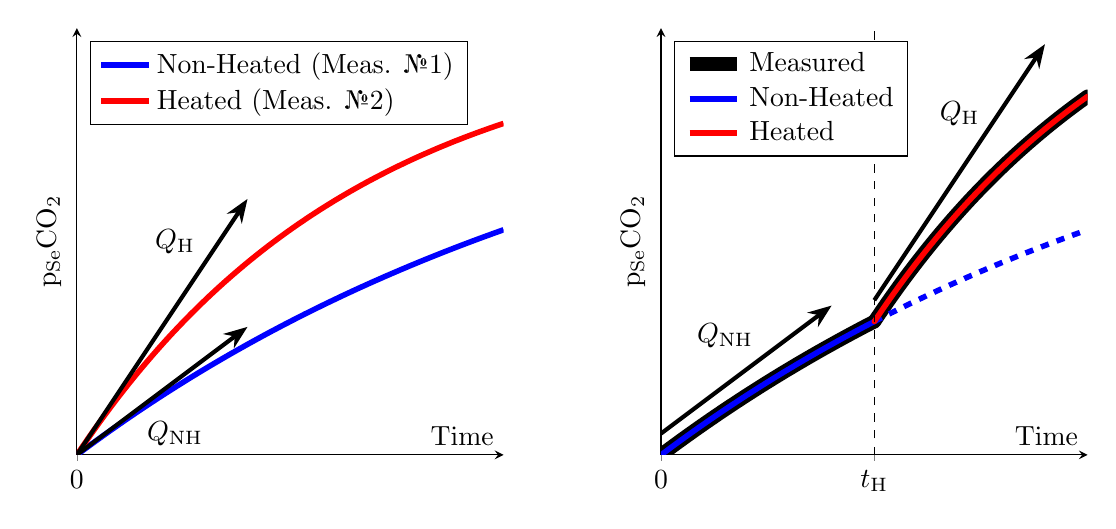
\begin{tikzpicture}
	\begin{groupplot}[group style={group size=2 by 1, horizontal sep=2cm},height=7cm, width=7cm]
		%
		% First plot
		%
		\nextgroupplot[
			axis lines = left,
			xlabel = Time,
			ylabel = p$_{\text{Se}}$CO$_2$,
			xmin=0,	xmax=10,
			ymin=0,	ymax=1,
			xtick={0},
			xticklabels={$0$},
			xlabel style = {at={(axis description cs:1,0)},anchor=south east},
			ytick=\empty,
			legend entries={Non-Heated (Meas. №1), Heated (Meas. №2)},
			legend style={at={(0.03,0.97)},anchor=north west},
			legend cell align={left},
			]
			\addplot[color=blue,
			domain=0:10,
			samples=200,
			line width=2pt,
			]{1-exp(-0.075*x)};
			\addplot[color=red,
			domain=0:10,
			samples=200,
			line width=2pt,,
			]{1-exp(-0.15*(x))};
			\draw[-{Stealth[length=3mm]}, line width=1.5] (axis cs:0, 0) -- (axis cs:4, 4*\mytau);
			\draw[-{Stealth[length=3mm]}, line width=1.5] (axis cs:0, 0) -- (axis cs:4, 2*4*\mytau);
			\node[align=center] at (2.3,0.5) {$Q_\text{H}$};
			\node[align=center] at (2.3,0.05) {$Q_\text{NH}$};
		%
		% Second Plot
		%
		\nextgroupplot[
		axis lines = left,
		xlabel = Time,
		ylabel = p$_{\text{Se}}$CO$_2$,
		xmin=0,	xmax=10,
		ymin=0,	ymax=1,
		xtick={0,5},
		xticklabels={$0$,$t_\text{H}$},
		xlabel style = {at={(axis description cs:1,0)},anchor=south east},
		ytick=\empty,
		legend entries={Measured, Non-Heated, Heated},
		legend style={at={(0.03,0.97)},anchor=north west},
		legend cell align={left},
		]
		% Fake plots for straight legend
		\addplot[color=black,
		domain=0:5,
		samples=200,
		line width=5pt,
		]coordinates {
			(-0.1,-0.1)
		};
		\addplot[color=blue, 
		domain=0:5,
		samples=200,
		line width=2pt,
		]coordinates {
			(-0.1,-0.1)
		};
		\addplot[color=red,
		domain=5:10,
		samples=200,
		line width=2pt,,
		]coordinates {
			(-0.1,-0.1)
		};
		%
		\addplot[color=black,line cap=round,
		domain=0:5,
		samples=200,
		line width=5pt,
		]{1-exp(-\mytau*x)};
		\addplot[forget plot, color=black,line cap=round,
		domain=5:10,
		samples=200,
		line width=5pt,
		]{1-exp(-2*\mytau*(x-5))+1-exp(-\mytau*5)};
		\addplot[color=blue, line cap=round,
		domain=0:5,
		samples=200,
		line width=2pt,
		]{1-exp(-\mytau*x)};
		\addplot[forget plot, color=blue,
		/tikz/dashed,
		domain=5:10,
		samples=200,
		line width=2pt,
		]{1-exp(-\mytau*x)};
		\addplot[color=red, line cap=round,
		domain=5:10,
		samples=200,
		line width=2pt,,
		]{1-exp(-2*\mytau*(x-5))+1-exp(-5*\mytau)};
		\addplot+ [ycomb, /tikz/dashed, black] coordinates {(5, 100)};
		\draw[-{Stealth[length=3mm]}, line width=1.5] (axis cs:0, 0+0.05) -- (axis cs:4, 4*\mytau + 0.05);
		\draw[-{Stealth[length=3mm]}, line width=1.5] (axis cs:5, {1-exp(-5*\mytau) + 0.05}) -- (axis cs:9, {1-exp(-5*\mytau) + 2*\mytau*(9-5) + 0.05});
		\node[align=center] at (7.0,0.8) {$Q_\text{H}$};
		\node[align=center] at (1.5,0.28) {$Q_\text{NH}$};
	\end{groupplot}
\end{tikzpicture}
\end{document}